% =====================================================================
%  fig-three-paths.tex  —  editable TikZ source for the Background
%  figure "Three paths out of coal".
%
%  This is the canonical source for the figure. Built from
%  concept2_tikz_spec.md; concept2_three_paths.pdf is the visual
%  reference. Colours and type (Source Sans 3) follow the research-
%  highlight design system.
%
%  BUILD (produces a vector PDF next to this file):
%      pdflatex fig-three-paths.tex
%  The research highlight reads that PDF from this directory, so no
%  copy step is needed — rebuild here and re-render the .qmd.
%
%  CANVAS & SCALING
%  Coordinates below are the spec's 560x372 artboard units at 0.75pt per
%  unit, with y negated (the spec measures y downward from the top-left).
%
%  There is deliberately no \useasboundingbox: standalone crops tight to
%  the drawn content, so the figure carries no margin of its own. That is
%  what lets the wrapped figure's title sit level with the first line of
%  Background text, matching the EPA compliance highlight. Adding an
%  artboard-sized bounding box reinstates the spec's 24-unit margins and
%  drops the title ~5pt below the text line.
%
%  Type sizes are canvas-relative: \includegraphics[width=W] scales
%  everything uniformly. Change the width in the .qmd, not here.
%
%  To edit: change the labels, coordinates, or colours below and rebuild.
% =====================================================================
\documentclass[border=0pt]{standalone}
\usepackage[T1]{fontenc}
\usepackage[default]{sourcesanspro}   % same typeface as the document
\renewcommand{\familydefault}{\sfdefault}
\usepackage{microtype}                % provides \textls letterspacing
\usepackage{sansmath}                 % keeps $\approx$ sans, not Computer Modern
\usepackage{tikz}
\usetikzlibrary{arrows.meta}

% The only math in the figure is the approx sign; keep it in the sans face
% so the spec's "no serif anywhere" holds.
\newcommand{\apx}{{\sansmath$\approx$}}

% ---- palette -------------------------------------------------------
% Mirrored from formats/research-highlight/_style.tex. A standalone
% document cannot see that file, so these are duplicated here; keep the
% hex values in sync if the design system changes.
\definecolor{accentred}{HTML}{641111} % title, path-box headers
\definecolor{boxred}{HTML}{8C2826}    % the two filled anchor boxes
\definecolor{boxtext}{HTML}{EEF1EA}   % text on those boxes
\definecolor{body}{HTML}{33352C}      % path-box body text
\definecolor{cite}{HTML}{6E6D61}      % italic result captions
\definecolor{muted}{HTML}{50534A}     % subtitle, arrows
\definecolor{warmrule}{HTML}{D8D2C2}  % divider + neutral box outlines
\definecolor{paper}{HTML}{FAF8F1}     % neutral box fill

\begin{document}
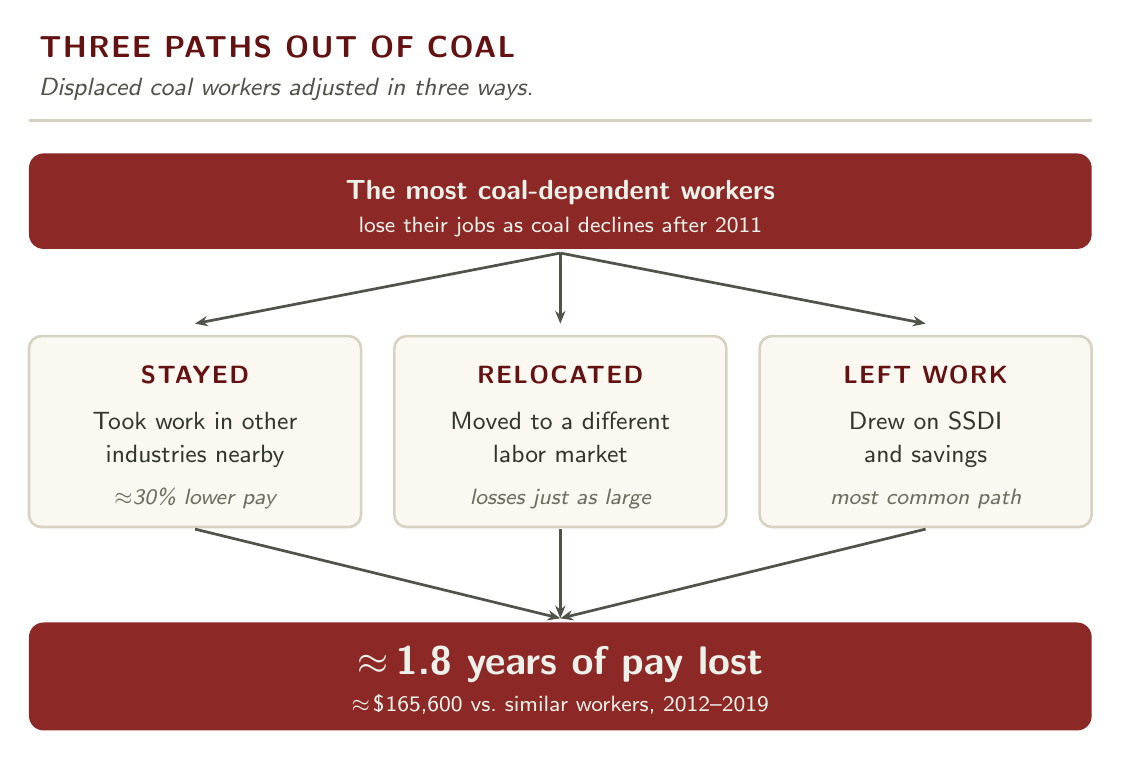
\begin{tikzpicture}[x=0.75pt, y=0.75pt,
  % --- boxes ---
  anchorbox/.style={rounded corners=5.25pt, fill=boxred, draw=none},
  pathbox/.style={rounded corners=4.5pt, fill=paper, draw=warmrule,
                  line width=0.95pt},
  % --- arrows ---
  arr/.style={muted, line width=0.98pt,
              -{Stealth[length=4.6pt, width=3.7pt]}}]

% ---------------------------------------------------------------------
% TITLE BLOCK
% ---------------------------------------------------------------------
\node[anchor=base west, accentred, font=\bfseries\fontsize{10.5pt}{12pt}\selectfont]
  at (24,-30) {\textls[40]{\MakeUppercase{Three paths out of coal}}};
\node[anchor=base west, muted, font=\itshape\fontsize{9pt}{11pt}\selectfont]
  at (24,-48) {Displaced coal workers adjusted in three ways.};
\draw[warmrule, line width=0.95pt] (24,-60) -- (536,-60);

% ---------------------------------------------------------------------
% TOP ANCHOR BOX — the shock
% ---------------------------------------------------------------------
\node[anchorbox, minimum width=384pt, minimum height=34.5pt] at (280,-99) {};
\node[anchor=base, boxtext, font=\bfseries\fontsize{9.75pt}{11pt}\selectfont]
  at (280,-98) {The most coal-dependent workers};
\node[anchor=base, boxtext, font=\fontsize{8.25pt}{10pt}\selectfont]
  at (280,-114) {lose their jobs as coal declines after 2011};

% ---------------------------------------------------------------------
% THE THREE PATHS
% ---------------------------------------------------------------------
% Box A — stayed
\node[pathbox, minimum width=120pt, minimum height=69pt] at (104,-210) {};
\node[anchor=base, accentred, font=\bfseries\fontsize{8.62pt}{10pt}\selectfont]
  at (104,-187) {\textls[50]{\MakeUppercase{Stayed}}};
\node[anchor=base, body, font=\fontsize{9pt}{11pt}\selectfont]
  at (104,-209) {Took work in other};
\node[anchor=base, body, font=\fontsize{9pt}{11pt}\selectfont]
  at (104,-225) {industries nearby};
\node[anchor=base, cite, font=\itshape\fontsize{8.25pt}{10pt}\selectfont]
  at (104,-245) {\apx30\% lower pay};

% Box B — relocated
\node[pathbox, minimum width=120pt, minimum height=69pt] at (280,-210) {};
\node[anchor=base, accentred, font=\bfseries\fontsize{8.62pt}{10pt}\selectfont]
  at (280,-187) {\textls[50]{\MakeUppercase{Relocated}}};
\node[anchor=base, body, font=\fontsize{9pt}{11pt}\selectfont]
  at (280,-209) {Moved to a different};
\node[anchor=base, body, font=\fontsize{9pt}{11pt}\selectfont]
  at (280,-225) {labor market};
\node[anchor=base, cite, font=\itshape\fontsize{8.25pt}{10pt}\selectfont]
  at (280,-245) {losses just as large};

% Box C — left work
\node[pathbox, minimum width=120pt, minimum height=69pt] at (456,-210) {};
\node[anchor=base, accentred, font=\bfseries\fontsize{8.62pt}{10pt}\selectfont]
  at (456,-187) {\textls[50]{\MakeUppercase{Left work}}};
\node[anchor=base, body, font=\fontsize{9pt}{11pt}\selectfont]
  at (456,-209) {Drew on SSDI};
\node[anchor=base, body, font=\fontsize{9pt}{11pt}\selectfont]
  at (456,-225) {and savings};
\node[anchor=base, cite, font=\itshape\fontsize{8.25pt}{10pt}\selectfont]
  at (456,-245) {most common path};

% ---------------------------------------------------------------------
% BOTTOM ANCHOR BOX — the shared outcome
% ---------------------------------------------------------------------
\node[anchorbox, minimum width=384pt, minimum height=39pt] at (280,-328) {};
\node[anchor=base, boxtext, font=\bfseries\fontsize{13.5pt}{15pt}\selectfont]
  at (280,-327) {\apx\,1.8 years of pay lost};
\node[anchor=base, boxtext, font=\fontsize{8.25pt}{10pt}\selectfont]
  at (280,-345) {\apx\,\$165,600 vs.\ similar workers, 2012--2019};

% ---------------------------------------------------------------------
% ARROWS — fan out from the shock, funnel in to the outcome.
% The fan-then-funnel is the point: three exits, one outcome.
% ---------------------------------------------------------------------
\draw[arr] (280,-124) -- (104,-158);
\draw[arr] (280,-124) -- (280,-158);
\draw[arr] (280,-124) -- (456,-158);

\draw[arr] (104,-257) -- (280,-300);
\draw[arr] (280,-257) -- (280,-300);
\draw[arr] (456,-257) -- (280,-300);

\end{tikzpicture}
\end{document}
